\documentclass{article}
\usepackage[utf8]{inputenc}
\usepackage[margin=1in]{geometry}
\usepackage{graphicx}
\usepackage{longtable}
\usepackage{array}
\usepackage{titlesec}
\usepackage{lipsum}
\usepackage{enumitem}
\usepackage{hyperref}

\usepackage{ragged2e} % For better text justification inside cells

% \captionsetup{justification=centering}

\usepackage{subcaption} 
\usepackage{float} % Required for the H float option

% Wrapping text in table cells


% Column types for clean formatting
\newcolumntype{L}[1]{>{\raggedright\arraybackslash}m{#1}} % Vertically centered, left-aligned
\newcolumntype{P}[1]{>{\raggedright\arraybackslash}p{#1}} % Top-align, wrapped text




% Section formatting
\titleformat{\section}{\large\bfseries}{\thesection.}{1em}{}

\title{\textbf{ETL Project Proposal}}
\author{Nishan Khanal \\
Data Engineering}
\date{\today}

\begin{document}

\begin{titlepage}
    % \vfill
    \centering
    %Make the following image centered vertically
    \vspace*{2in}
    % \includegraphics[width=0.25\textwidth]{images/postgres.png}
    
    {\LARGE
    \vspace{1in}
    End to End Pipeline for Chicago Crime Data \\ 
    
    \vspace{0.5cm}
    Data Engineering\\
    \vspace{0.5cm}
    }% Documentation}\\
    \Large{
        \vskip1cm
        \today\\
        \vskip0.3cm
        Nishan Khanal\\
    }
       
\end{titlepage}

\tableofcontents
\newpage

% \maketitle

\section{Project Overview}
There are certain datasets for which we have up-to-date information in a single large file. However, if the instances in these datasets have temporal features and if the instances are bound to occur in the future, continuous integration is required to incorporate the future instances. I’ve decided to do this for the Chicago crime dataset. As of April 4, 2025, the dataset contains the crime records till “March 26, 2025”. It is not suitable to download the entire dataset when up-to-date information is required, which is better suited for fetching smaller, newer portions through APIs. Using the API for fetching the entire dataset is also not suitable, as the dataset is huge, and we might exceed the rate limit quickly. The approach I suggest is to fetch the entire dataset once and use APIs to update the data as we move forward.

\section{Data Source Selection}
\subsection{Dataset Choice}
I’ve selected the \textbf{Chicago Crime Dataset} for this project. This dataset contains the reported incidents of crime in the City of Chicago from 2001 to present (minus the most recent 7 days). The dataset is deidentified in the spatial domain, i.e, the addresses are only accurate to the block level. This dataset will be helpful for analyzing crime patterns, and trends, and for predicting future crime hotspot. 
I will also be using supplementary datasets. I will be using the \textbf{Chicago Community Areas dataset}, which will aid in the visualization of the crime location in different communities. This dataset contains geographic information (GIS) about the different communities in Chicago.
\subsection{Dataset Description}
The Chicago Crime dataset contains $\sim$ 8 million reported incidents and the following columns:
\begin{itemize}[leftmargin=2em]
    \item \textbf{ID:} Unique identifier for each incident
    \item \textbf{Case Number:} Unique case number for each incident
    \item \textbf{Date:} Date and time of the incident
    \item \textbf{Block:} Block where the incident occurred
    \item \textbf{Primary Type:} Type of crime (e.g., theft, assault)
    \item \textbf{Description:} Description of the crime
    \item \textbf{Location Description:} Description of the location where the incident occurred
    \item \textbf{Arrest:} Indicates whether an arrest was made
    \item \textbf{Domestic:} Indicates whether the incident was domestic in nature
    \item \textbf{Beat:} Police beat where the incident occurred
    \item \textbf{District:} Police district where the incident occurred
    \item \textbf{Ward:} City ward where the incident occurred
    \item \textbf{Community Area:} Community area where the incident occurred
    \item \textbf{FBI Code:} FBI classification code for the crime
    \item \textbf{X Coordinate:} X coordinate of the incident location
    \item \textbf{Y Coordinate:} Y coordinate of the incident location
    \item \textbf{Year:} Year of the incident
    \item \textbf{Updated On:} Date and time when the record was last updated
    \item \textbf{Latitude:} Latitude of the incident location
    \item \textbf{Longitude:} Longitude of the incident location
    \item \textbf{Location:} Location of the incident (latitude and longitude)
\end{itemize}

\noindent The Chicago Community Areas dataset contains 77 rows - one for each community - and the following columns:
\begin{itemize}[leftmargin=2em]
    \item \textbf{community area:} Unique identifier for each community area
    \item \textbf{shape\_area:} Area of the community shape
    \item \textbf{perimeter:} Perimeter of the community shape
    \item \textbf{area\_num\_1:} Area id
    \item \textbf{area\_numbe:} Area number
    \item \textbf{comarea\_id:} Community area ID
    \item \textbf{comarea:} Community area name
    \item \textbf{shape\_len:} Length of the community shape
    \item \textbf{geometry:} Geometry of the community area (multipolygon)
\end{itemize}


\subsection{Selection Criteria and justification}
While just downloading the large dataset would not carry appropriate weight in the extract phase of the ETL pipeline, my proposed approach of using an API to update the data periodically ensures that the extract phase is complex enough. As for the transformation, there are going to be a lot of steps involved, like handling missing values, mainly through imputation leveraging the help of a secondary dataset, removing outliers, etc., which will satisfy the complexity criteria of the project. And, for the Loading phase, I’ll create an appropriate schema in PostgreSQL and load the data there. 


\section{Technology \& Tool Stack}
\subsection{ETL Tools \& Platforms}
\begin{itemize}[leftmargin=2em]
    \item \textbf{Python:} for accessing the dataset and implementing transformation logic. I plan on using the following libraries. (Some additional libraries may also be used along the way) 
    \begin{itemize}[leftmargin=2em]
        \item \textbf{pandas:} for data loading, manipulation and analysis
        \item \textbf{NumPy:} for numerical operations
        \item \textbf{sodapy:} for accessing the Chicago crime dataset API
        \item \textbf{psycopg2:} for database connection
        \item \textbf{geopandas:} for geospatial data manipulation
    \end{itemize}
    \item \textbf{Apache Airflow/ Cron}: I'm planning to use Apache Airflow for workflow automation when accessing new data from the API and transforming it. I might end up just using cron if the workflow is simple.
\end{itemize}

\subsection{Database \& Storage Options}
\begin{itemize}[leftmargin=2em]
    \item \textbf{PostgreSQL:} I will load the transformed data into a local PostgreSQL database, which will then be used for analysis. 
\end{itemize}

\subsection{Visualization}
\begin{itemize}
    \item \textbf{Matplotlib/Seaborn:} for creating static, animated and interactive visualizations in Python.
    \item \textbf{GCP Looker Studio:} for creating interactive dashboards and reports.
\end{itemize}

\section{Implementation Approach}

Figure \ref{fig:workflow} shows the ETL workflow. The data will be extracted from the Chicago Crime dataset and the Chicago Community Areas dataset. The data will be transformed through cleaning, normalization, enrichment, and data type conversion. The transformed data will then be loaded into a PostgreSQL database. Finally, the data will be analyzed and visualized using Python libraries and GCP Looker Studio.
\begin{figure}[h]
    \centering
    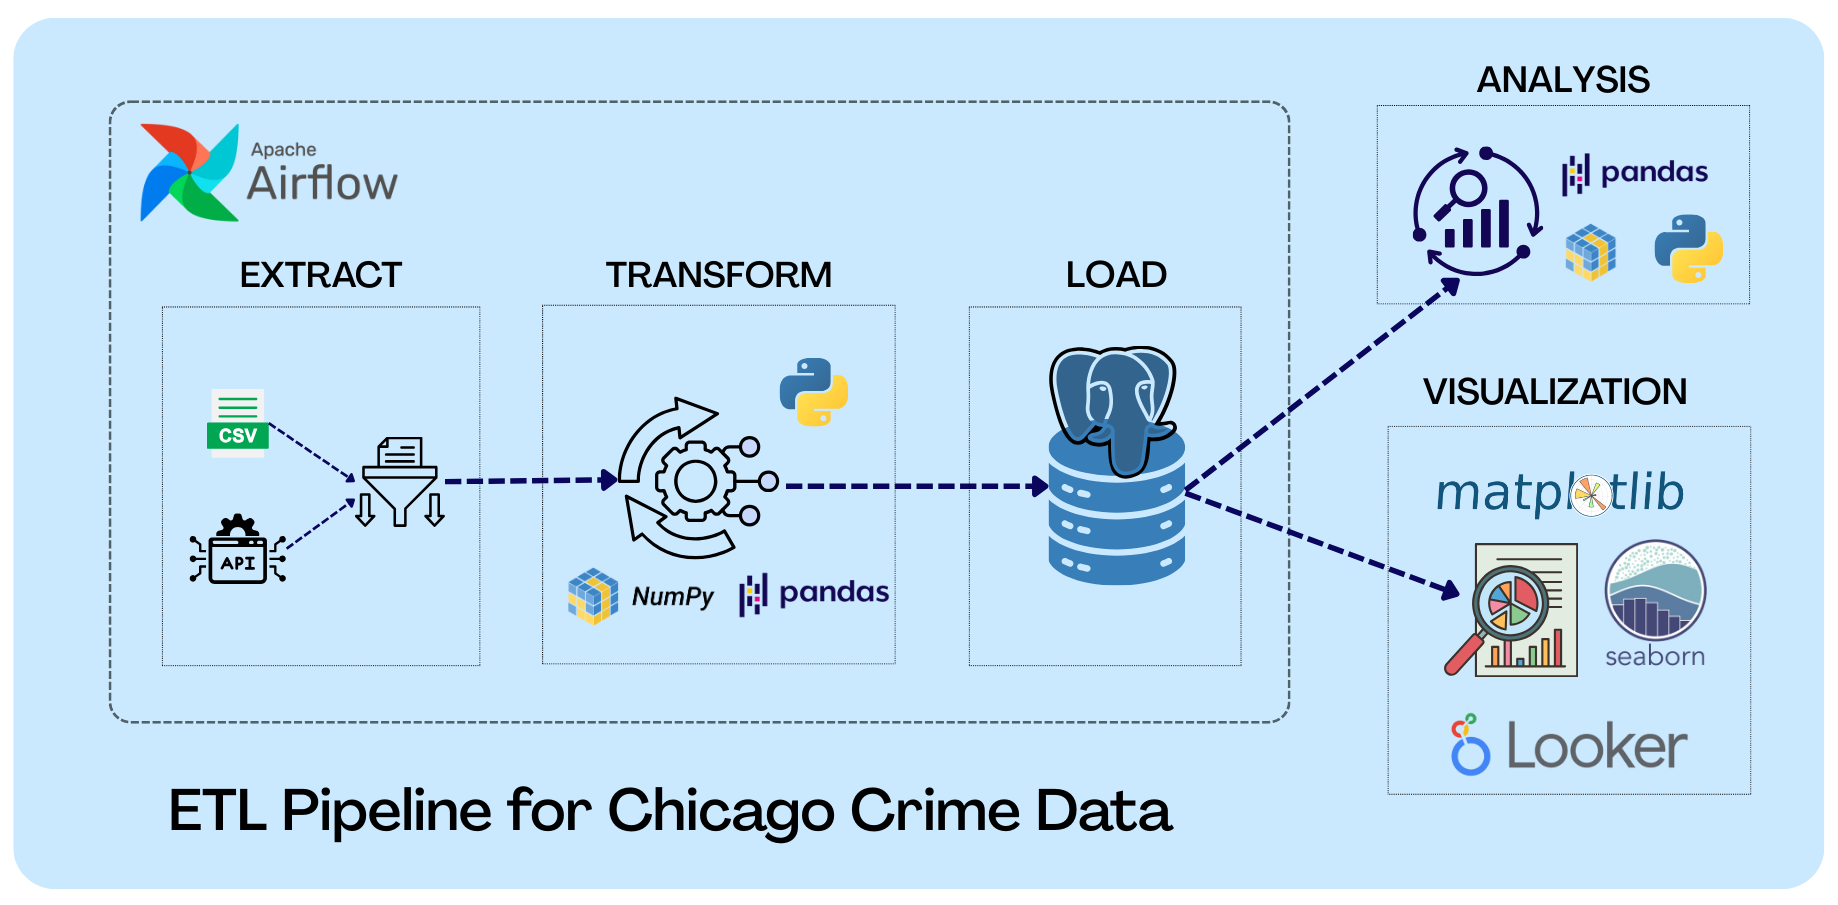
\includegraphics[width=1\textwidth]{images/workflow.png}
    \caption{ETL Workflow}
    \label{fig:workflow}
\end{figure}

\subsection{Data Extraction}
The large crime dataset from 2001 to the present will be downloaded as a single CSV file from the link. This data will be updated through the use of the Chicago API, powered by Socrata. The supplementary Chicago Community Areas dataset will be downloaded as a single SHP/Geojson file, which includes the boundary data as multipolygons for each community. 

The data extraction from the API will be automated and scheduled through the use of Apache Airflow or Cron.

\subsection{Data Transformation}
\begin{itemize}
    \item \textbf{Cleaning:} In this phase, the missing values and outliers will be handled, and any duplicates will be removed. The columns will be converted to appropriate data types. The large dataset and the data coming in from the API have different names for columns, which will be handled by using a standardized naming convention. More specifically, in the cleaning phase, the missing values of the community areas will be imputed with the help of the Chicago Community Areas dataset by determining which crime location falls within which community by performing a spatial join (provided by geopandas).
\item  \textbf{Normalization:} The data will be stored as is. i.e. De-normalized. Since this database will be mostly used for querying rather than for transaction processing,                                                                                                                                                                                                                                                                                                                                                                                                                                                                                                                              I think a 
    \item \textbf{Data Type Conversion:} The data types will be converted to appropriate types. For example, the date column will be converted to a date type, and the categorical columns will be converted to categorical types.denormalized table would be better.
    \item \textbf{Enrichment:} The main dataset will be accompanied by the Chicago Community Areas dataset. Aggregation will be mainly performed during the analysis phase. Temporal information will be decomposed for easy integration with another dataset in the future that only has aggregated information. I will store the data at the most granular level so that the aggregation can be done according to the purpose of the analysis.
\end{itemize}

\subsection{Data Loading}
\begin{itemize}[leftmargin=2em]
    \item \textbf{Database Selection:} I first plan to load the data into a local PostgreSQL database. I chose a relational database because the dataset under consideration has a tabular structure.
    \item \textbf{Schema Design:} Since this dataset is huge and will be used mainly for analysis, it will be denormalized.
    \item \textbf{Loading Method:} psycopg2 will be used to make the connection, and bulk insert will be performed after the transformation.
\end{itemize}

\subsection{Data Analysis \& Visualization}
\begin{itemize}
    \item \textbf{Exploratory Data Analysis (EDA):} Jupyter Notebook, aided by Python libraries like matplotlib, seaborn, and plotly, will be used to explore data patterns, distributions, and correlations.
    \item \textbf{Visualization:} I will create visualizations using matplotlib and seaborn. I will also use Google Looker Studio to create interactive dashboards.
\end{itemize}

\section{Project Timeline}

Figure \ref{fig:gantt-chart} shows the Gantt chart of the project timeline. The project is divided into four weeks, with each week focusing on a specific milestone. This is further described in table \ref{tab:project-timeline}
\begin{longtable}{|L{2cm}|L{3cm}|L{10cm}|}
    \hline 
    \textbf{Week} & \textbf{Milestone} & \textbf{Description} \\
    \hline
    Week 1 & Proposal Submission \& Planning &
    
    - Submit the project proposal document, clearly outlining the data source, technology stack, tools, and implementation strategy\newline
    - Finalize the dataset selection\newline
    - Conduct initial data exploration\newline
    - Outline ETL workflow structure (diagram or notes) to inform Week 2 development\newline
    - Document the process
       \\
    \hline
    Week 2 & Environment Setup \& Initial Pipeline &
    
    - Set up development tools: Python environment, VS Code, and Git repo.\newline
    - Begin scripting for data extraction (from API, file download, or scraping)\newline
    - Implement and test initial transformation logic (cleaning, basic normalization)\newline
    - Set up an orchestration tool (Airflow) to schedule data extraction jobs\newline
    - Document the process
    \\
    \hline
    Week 3 & Complete ETL Integration &
    
    - Expand transformation logic with enrichment and advanced cleaning/imputation tasks\newline
    - Finalize data loading into the target storage system (PostgreSQL)\newline
    - Design database schema and apply indexing\newline
    - Begin testing for pipeline performance and data accuracy\newline
    - Create automated workflows for recurring or batch ingestion\newline
    - Document the process
    \\
    \hline
    Week 4 & Visualization, Monitoring, \& Final Documentation &
    
    - Create interactive dashboards using open-source BI tools (Metabase, Superset) or GCP’s Looker Studio (if applicable)\newline
    - Conduct final data quality checks and optimize transformation scripts\newline
    - Document all implementation steps, architectural decisions, and visual outputs\newline
    - Finalize project for submission/presentation, including README, code, dashboard links, and diagrams
    \\
    \hline
    \caption{Project Timeline}
    \label{tab:project-timeline}
\end{longtable}

\begin{figure}[H]
    \centering
    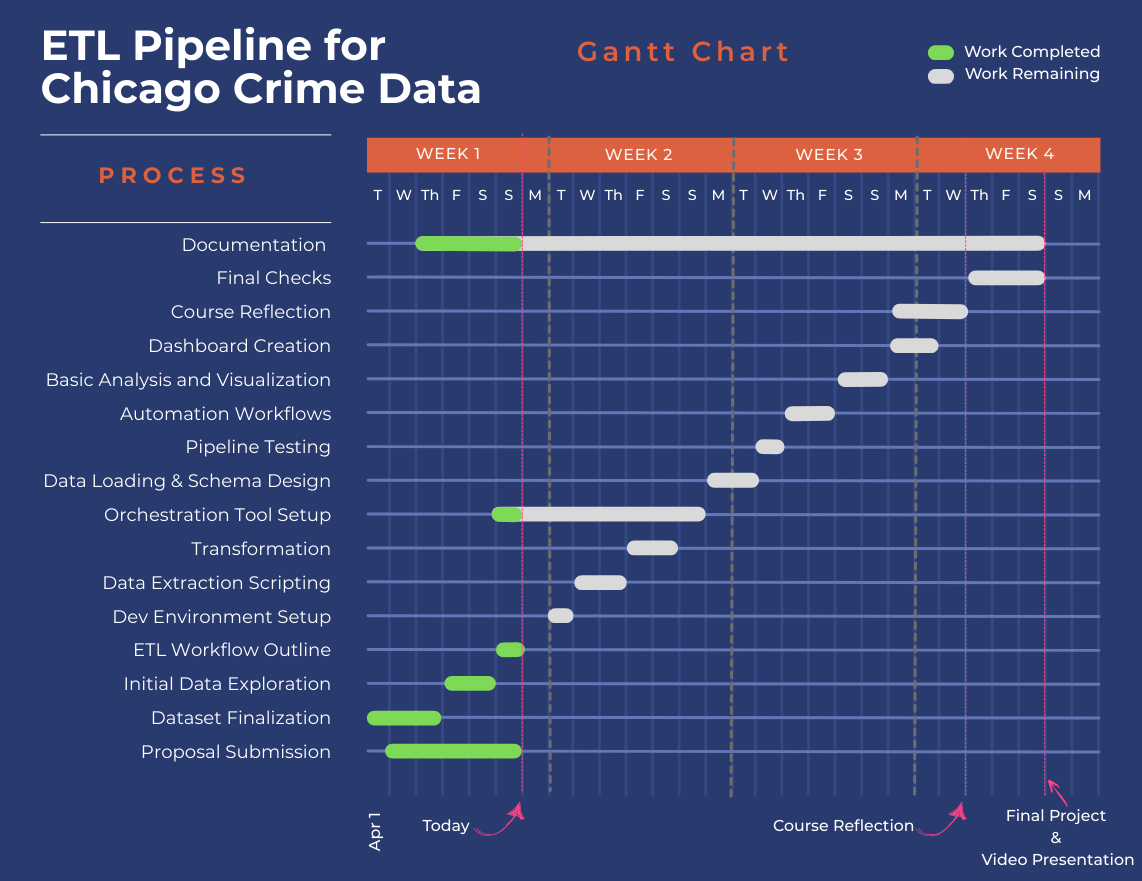
\includegraphics[width=1\textwidth]{images/gantt-chart.png}
    \caption{Gantt Chart of the Project Timeline}
    \label{fig:gantt-chart}
\end{figure}



\section{Expected Challenges}
I am anticipating the following challenges. I’ve also proposed some strategies to overcome those challenges. 


\begin{longtable}{|L{3cm}|L{6cm}|L{6cm}|}
    \hline
    \textbf{Challenge} & \textbf{Description} & \textbf{Proposed Strategy} \\
    \hline
    \endfirsthead

    Data Quality Issues & With the preliminary analysis, I’ve found that the data contains missing values, outliers, and invalid values. & I’ll programmatically impute missing values for community\_id from another dataset and remove instances that have invalid values. \\
    \hline
    API Issues & This is a public and freely available dataset, so with frequent requests, I can face a rate limitation. & All the available data till present will be downloaded as a static file. I plan to update the data daily, which won’t have too many records, reducing the number of requests to the server. \\
    \hline
    Setting Environments with New Tools & I may face a problem in setting up Apache Airflow as I’ve never used it before. & I’ll start familiarizing myself with new tools early on, as displayed on the Gantt chart. \\
    \hline
    Performance and Scalability & As the dataset contains $\sim$ 8 million rows, I might face some performance issues. & If such issues arise, I’ll look into Spark and cloud-based processing. \\
    \hline
    Visualization Clarity and Usability & Creating visualizations that clearly convey insights without overwhelming users can be difficult. & I’ll keep in mind that the visualization should be accessible to both technical and non-technical users. I’ll focus on key performance indicators pertinent to my dataset. \\
    \hline
    Looker Studio Connection to Local Database & I may face issues connecting Looker Studio to my local PostgreSQL database. & I’ll look into the documentation and community forums for solutions. \\
    \hline
    \caption{Expected Challenges}
    \label{tab:challenges}
\end{longtable}

% \section*{References}
\addcontentsline{toc}{section}{References}
% \nocite{pandas,airflow,geopandas,sodapy}
\nocite{*}
\bibliographystyle{plain}
\bibliography{references}


\end{document}